\chapter{曲线运动}\label{chp:curve_movement}
到现在为止,我们只讨论了与物体的直线运动有关的运动学和动力学问题。
除直线运动外,我们还常常遇到曲线运动。
抛出的石子,是沿着一条曲线落地的(\cref{fig:4-1})。
各种车辆拐弯时所做的运动,地球、月球沿轨道的运动,也都是曲线运动。
曲线运动比直线运动复杂些,这一章我们要进一步运用已有的运动学和动力学知识来研究曲线运动。

\begin{figure}
  \includegraphics{4-1.pdf}
  \caption{水平扔出的石子沿曲线运动}\label{fig:4-1}
\end{figure}

\section{曲线运动}
\subsection{曲线运动的速度方向}
曲线运动跟直线运动的明显区别是它的速度方向在时刻改变。那么,在曲线运动中,速度的方向是怎样确定的呢?

\begin{figure}
  \includegraphics{4-2.pdf}
  \caption{火星沿砂轮的切线飞出}\label{fig:4-2}
\end{figure}

我们在砂轮上磨刀具(\cref{fig:4-2}),可以看到,刀具与砂轮接触处有火星沿砂轮的切线飞出。
这些火星是刀具与砂轮磨出的炽热的微粒,它们被分离出来时,由于惯性而以分离时具有的速度做直线运动,因此,火星飞出的方向就表示砂轮上跟刀具接触处的速度方向。
如果沿着砂轮圆周移动刀具,可以看到,在任何位置,火星都从接触处沿砂轮的切线飞出。
让撑开的带有水的伞绕着伞柄旋转,也可以看到水滴是沿着伞边各点所画圆周的切线飞出的。

从这些和类似的观察知道,\emph{曲线运动中速度的方向是时刻改变的,质点在某一点(或某一时刻)的即时速度的方向在曲线的这一点的切线上}(\cref{fig:4-3})。

\begin{figure}
  \includegraphics{4-3.pdf}
  \caption{曲线运动中某点的即时速度的方向在曲线的这一点的切线上}\label{fig:4-3}
\end{figure}

我们知道,速度是个矢量,既有大小,又有方向,不论速度的大小是否改变,只要速度的方向发生改变,就表示速度矢量发生了变化,也就是具有加速度。
曲线运动中速度的方向时刻在改变,所以\Concept{曲线运动是变速运动}。

\subsection{物体做曲线运动的条件}

物体在什么情况下才做曲线运动呢?
这个问题不难根据牛顿第二定律来说明.我们知道,物体的速度发生变化,有了加速度,是由外力引起的,加速度的方向总跟合外力的方向一致。
如果合外力的方向跟物体速度的方向在同一条直线上,产生的加速度的方向也在这条直线上,这时只改变速度的大小,不改变速度的方向,速度的方向仍旧在这条直线上,物体就做直线运动。
如果合外力的方向跟速度的方向不在一条直线上,而是成一角度,那么一般说来,合外力就不但改变速度的大小,而且改变速度的方向,物体就做曲线运动。

水平抛出的石子,由于所受的重力跟速度的方向不在一条直线上,所以石子做曲线运动(\cref{fig:4-4})。

\begin{figure}
  \includegraphics{4-4.pdf}
  \caption{}\label{fig:4-4}
\end{figure}
 
\begin{Practice}
\begin{question}
  \item 汽车以恒定的速率 \qty{2}{min} 绕广场行驶一周,汽车每行驶半周速度方向改变多少度?汽车每行驶 \qty{10}{s} 速度改变多少度?画出汽车在相隔 \qty{10}{s} 的两个位置处的速度矢量。
  \item 举出两个实例,说明物体做曲线运动的条件。
  \item 某人骑着自行车以恒定的速率驶过一段弯路,自行车进行的是匀速运动还是变速运动?为什么?
\end{question}
\end{Practice}

\section{运动的合成和分解}
研究比较复杂的运动时,常常把这个运动看作是两个或几个比较简单的运动组成的,使问题变得容易研究。
作为研究曲线运动的准备,我们先讨论一下运动的合成和分解。

轮船渡河的运动可以看作是由两个运动组成的。
假如河水不流动,而轮船在静水中沿 $AB$ 方向行驶,那么经过一段时间轮船将从 $A$ 点运动到 $B$ 点(\cref{fig:4-5})。
假如轮船没有开动,而河水流动,那么轮船被河水冲向下游,经过相同一段时间,轮船将从 $A$ 点运动到 $A'$ 点。
现在轮船在流动的河水中行驶,它同时参与上述两个运动,经过这段时间将从 $A$ 点运动到 $B'$ 点。
轮船从 $A$ 点到 $B'$ 点的运动,就是上述两个分运动的合运动。

\begin{figure}
  \includegraphics{4-5.pdf}
  \caption{轮船渡河的运动}\label{fig:4-5}
\end{figure}

既然一个运动可以看作是由分运动组成的,那么,已知分运动的情况,就可以知道合运动的情况,由于位移是矢量,已知分运动在一段时间内发生的位移,应用平行四边形法则就可以求出合运动的位移。
同样,由于速度和加速度都是矢量,已知分运动在某一时刻的速度和加速度,应用平行四边形法则就可以求出合运动在那一时刻的速度和加速度。
例如,在上面轮船渡河的例子中,如果知道了轮船在静水中的速度 $v_1$ 的大小和方向,以及河水流动的速度 $v_2$ 的大小和方向,应用平行四边形法则,就可以求出轮船合运动的速度 $v$(\cref{fig:4-6}),这种已知分运动求合运动,叫做\Concept{运动的合成}。

\begin{figure}
  \includegraphics{4-6.pdf}
  \caption{速度的合成}\label{fig:4-6}
\end{figure}

反过来,已知合运动情况,应用平行四边形法则,也可以求出分运动的情况。
例如,飞机以 \qty{300}{km/h} 的速度斜向上飞行,方向与水平面成 \ang{30} 角,我们很容易求出飞机在水平方向和竖直方向的速度。
由于飞机斜向上飞行的运动可以看作是它在水平方向和竖直方向两个分运动的合运动,如\cref{fig:4-7} 把合运动的速度 $v$ 分解成水平方向和竖直方向的分速度 $v_x$ 和 $v_y$,它们就是这两个分运动的速度。
\[\begin{split}
v_x&=v\cos\ang{30}=\qty{260}{km/h},\\
v_y&=v\sin\ang{30}=\qty{150}{km/h}.\\
\end{split} \]

\begin{figure}
  \includegraphics{4-7.pdf}
  \caption{速度的分解}\label{fig:4-7}
\end{figure}

这种已知合运动求分运动,叫做\Concept{运动的分解}。

在\cref{fig:4-5} 轮船渡河的例子中,由于轮船在 $AB$ 方向是匀速行驶的,河水在 $AA'$ 方向是匀速流动的,轮船的两个分运动的速度矢量都是恒定的,轮船的合运动的速度矢量也是恒定的,所以合运动是匀速直线运动。
但一般来说,两个直线运动的合运动,并不一定都是直线运动。
在轮船渡河的例子中,如果轮船在 $AB$ 方向是加速行驶的,河水在 $AA'$ 方向的流动匀速的,那么轮船的合运动就不是直线运动,而是曲线运动了(\cref{fig:4-8})。

\begin{figure}
  \includegraphics{4-8.pdf}
  \caption{}\label{fig:4-8}
\end{figure}

一些常见的曲线运动往往可以分解为两个简单的直线运动。
下面我们将用运动的合成和分解来研究几种曲线运动。

\begin{Practice}
\begin{question}
  \item 降落伞在下落一定时间以后的运动是匀速的,没风的时候某跳伞员着地的速度是 \qty{5.6}{m/s},现庄有风,风使他以 \qty{4.0}{m/s} 的速度沿水平方向向东移动,他将以多大的速度着地?这个速度的方向怎样?
  \item 炮筒与水平方向成 \ang{60} 角,炮弹从炮口射出时的速度是 \qty{800}{m/s}。这个速度在竖直方向和水平方向的分速度各是多大?
  \item 小汽艇在静水中的速度是 \qty{12}{km/h},河水的流建是 \qty{6.0}{km/h}。如果驾驶员向着垂直于河岸的方向驾驶,小汽艇在河水中实际行驶的速度是多大?方向怎样?
\end{question}
\end{Practice}


\section{平抛物体的运动}
\subsection{平抛物体的运动} 
将物体用一定的初速度沿水平方向抛出去,物体所数的运动叫做\Concept{平抛运动}。
把桌上的小球打一下,使它有一个水平的初速度离开桌面,小球离开桌面后所做的曲线运动就是平抛运动。
在平抛运动中,物体受到跟速度方向成角度的重力(不考虑空气阻力),所以做曲线运动。

\begin{figure}
  \begin{minipage}[b]{0.55\linewidth}\centering
    \includegraphics{4-9.pdf}
    \caption{平抛运动的竖直分运动是自由落体运动}\label{fig:4-9}
  \end{minipage}%
  \begin{minipage}[b]{0.42\linewidth}\centering
    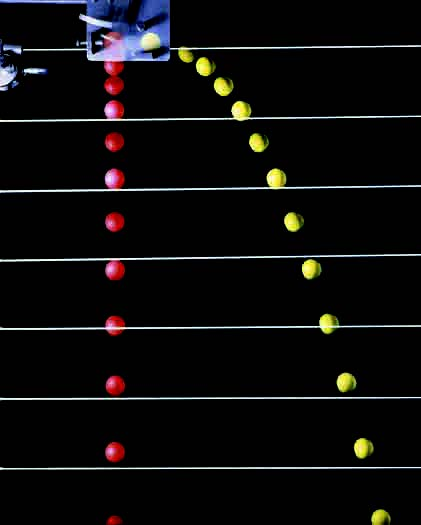
\includegraphics[scale=.6]{4-10.jpg}\par
    \footnotesize 照片是每隔 1/30\,\unit{s} 拍摄的,\\水平线间的距离是 \qty{15}{cm}
    \caption{平抛运动的闪光照片}\label{fig:4-10}
  \end{minipage}
\end{figure}

如\cref{fig:4-9} 所示,用小锤打击弹性金属片,使球 $A$ 向水平方向飞出,做平抛运动,同时球 $B$ 被放开,做自由落体运动。
实验表明,两球总是同时落地,这说明平抛运动在竖直方向上的运动是自由落体运动。
我们还可以用闪光照相的办法来更精细地研究这种实验。
\cref{fig:4-10} 是这种实验的闪光照片。
可以看出,尽管两球水平方向的运动不同,但它们在竖直方向的运动是相同的,即经过相同的时间下落相同的距离。
仔细测量平抛物体在水平方向的运动,可以证实这个运动是匀速的。
可见,平抛运动实际上是两个分运动的合运动:一个是在水平方向物体由于惯性而保持的匀速直线运动,其速度等于平抛物体的初速度;另一个是竖直方向物体在重力作用下的自由落体运动。

\subsection{平抛运动的公式} 
由于平抛运动是水平方向的匀速运动和竖直方向的自由落体运动的合运动,所以我们可以分别算出任何时刻 $t$ 物体的位置坐标 $x$ 和 $y$,取水平方向为 $x$ 轴,正方向与初速度 $v_0$ 的方向相同;取竖直方向为 $y$ 轴,正方向向下;取抛出点为原点。加速度方向与 $y$ 轴正方向相同,所以是正值,即 $a=g$。
物体在任何时刻 $t$ 的位置坐标可以由下面的公式求出:
\[\begin{split}
x&=v_0 t,\\
y&=\frac{1}{2}gt^2.
\end{split} \]
根据这两个公式求出任何时刻物体的位置,用平滑曲线把这些位置连起来,就得到平抛运动的轨迹。
这个轨迹是一条抛物线。
\cref{fig:4-11}是 $v_0= \qty{20}{m/s}$ 的平抛运动的轨迹。

\begin{figure}
  \begin{minipage}{0.45\linewidth}
  \begin{tblr}{colspec={X[c]X[c]X[c]},hline{2}=0.8pt}
    $t$ (\unit{s})& $x$ (\unit{m}) & $y$ (\unit{m}) \\
    1 & 20 & 5\\
    2 & 40 & 20\\
    3 & 60 & 45\\
    $\vdots$ & $\vdots$ & $\vdots$\\
  \end{tblr}
  \end{minipage}
  \begin{minipage}{0.52\linewidth}\centering
    \includegraphics{4-11.pdf}
  \end{minipage}
  \caption{平抛运动的运动轨迹($g=\qty{10}{m/s^2}$)}\label{fig:4-11}
\end{figure}

\begin{example}
飞机在 \qty{810}{m} 的高空中水平飞行,速度是 \qty{252}{km/h}。为了使飞机上落下的物体落在指定地点,应该在离开指定地点的水平距离多远的地方让物体落下?不计空气阻力。
\end{example}

\begin{solution}
从水平飞行的飞机上落下的物体做平抛运动,初速度就是飞机的飞行速度 $v_0= \qty{252}{km/h} = \qty{70}{m/s}$。物体开始下落的地方到落地点的水平距离 $x$ 可以用公式$x=v_0t$ 来计算。飞行时间 $t$ 可以从公式 $y=\dfrac{1}{2}gt^2$ 求出:
\[t=\sqrt{\frac{2y}{g}},\]
代入 $x=v_0 t$ 中得到:
\[\begin{split}
x&=v_0\sqrt{\frac{2y}{g}}\\
&= \qty{70}{m/s}  \times \sqrt{\frac{2\times \qty{810}{m}}{\qty{9.8}{m/s^2}}}=\qty{900}{m}.
\end{split} \]
即应该在离指定地点的水平距离是 \qty{900}{m} 的地方让物体落下,才能落在指定的地点。
\end{solution}

\begin{Practice}
下面各题都不考虑空气阻力。
\begin{question}
  \item 从一定高度水平抛出去的物体,它在空中飞行的时间是由什么决定的?抛射的水平距离又是由什么决定的?
  \item 从同一高度以不同的速度水平抛出两个质量不同的石子,下面的说法哪个对?
  \begin{tasks}
    \task 速度大的先着地;
    \task 质量大的先着地;
    \task 两个物体同时着地。
  \end{tasks}
  实际做一做,看你的判断是否正确。
  \item 从 \qty{1.6}{m} 高的地方水平射出一颗子弹,初速度是 \qty{700}{m/s},求这颗子弹飞行的水平距离。
  \item 一个小球从 \qty{1.0}{m} 高的桌面上水平抛出,落到地面的位置离开桌子的边缘 \qty{2.4}{m},小球离开桌子边缘时的初速度多大?
  \item 从 \qty{15}{m} 高的楼上以 \qty{1.0}{m/s} 的速度水平扔出一物体,此物体落地时的速度多大?方向是否与地面垂直?
\end{question}
\end{Practice}

\section{斜抛物体的运动}
\subsection{斜抛物体的运动} 
将物体用一定的初速度向斜上方抛出去,物体所做的运动叫做\Concept{斜抛运动}。
投出的标枪和手榴弹,向斜上方射出的子弹和炮弹,它们的运动都是斜抛运动。
在斜抛运动中,物体由于受到跟速度成角度的重力(不考虑空气阻力),所以做曲线运动。
做斜抛运动的物体先是沿着曲线上升,升到一个最高点,然后再沿着曲线下降,下面我们来具体研究斜抛物体的运动情况。

设物体以初速度 $v_0$ 向与水平方向成 $\theta$ 角的斜上方抛出(\cref{fig:4-12})。我们把 $v_0$ 分解为水平方向的分速度 $v_x=v_0\cos\theta$ 和竖直方向的分速度$v_y=v_0\sin\theta$。
这样,斜抛运动可以看作是下面两个分运动的合运动:一个是水平方向的匀速直线运动,速度等于 $v_x$;另一个是竖直上抛运动,初速度等于 $v_y$。
这样就可以应用匀速直线运动和竖直上抛运动的公式,来确定斜抛物体在任一时刻的位置。
我们选物体的抛出点为坐标原点;取水平方向为 $x$ 轴,正方向与初速度的方向成锐角;竖直方向为 $y$ 轴,正方向向上;加速度总与 $y$ 轴正方向相反,所以 $a=-g$。于是:物体在任一时刻的位置坐标
\[\begin{split}
x&=v_x t=v_0\cos\theta \cdot t,\\
y&=v_y t-\frac{1}{2}gt^2=v_0\sin\theta \cdot t-\frac{1}{2}gt^2.
\end{split} \]

根据这两个公式求出任何时刻物体的位置,用平滑曲线把这些位置连接起来,就得到斜抛运动的轨迹(\cref{fig:4-12})。这个轨迹也是一条抛物线。

\begin{figure}
  \includegraphics{4-12.pdf}
  \caption{斜抛运动}\label{fig:4-12}
\end{figure}

竖直上抛运动和平抛运动都可以看作斜抛运动的特殊情况,当抛射角 $\theta=\ang{90}$ 时,$v_x=0$, $v_y=v_0$,物体的运动就是竖直上抛运动。
当抛射角 $\theta =\ang{0}$ 时,$v_x=v_0$,$v_y=0$,从某一高度抛出的物体的运动就是平抛运动。

\subsection{射高和射程} 

在斜抛运动中,轨迹最高点的高度叫做射高 $Y$,物体被抛出的地点到落地点的水平距离叫做射程 $X$。怎样求射高和射程呢?斜抛物体的射高是由它的竖直方向的分运动决定的,求出初速度为 $v_y$ 的竖直上抛运动的最大高度,就得到了斜抛运动的射高。
在竖直上抛运动中,我们还计算过物体从被抛出到落回原地所用的时间 $T$。
求出物体在这个时间 $T$ 内在水平方向发生的位移,就得到了斜抛运动的射程。
这个时间 $T$ 也就是做斜抛运动的物体从被抛出到落地所用的时间,叫做飞行时间。

设斜抛物体的初速度为 $v_0$,抛射角为 $\theta$,利用竖直上抛运动的知识就可以求出飞行时间 $T$:
\[T=\frac{2v_y}{g}=\frac{2v_0\sin\theta}{g}.\]

求出竖直上抛分运动的最大高度就得到射高 $Y$:
\[Y=\frac{v^2_y}{2g}=\frac{v_0^2\sin^2\theta}{2g}.\]

已知飞行时间 $T$,代入公式 $x=v_0\cos\theta \cdot t$ 中就求出射程 $X$:
\[X=v_0\cos\theta \cdot T=\frac{2v_0^2\sin\theta \cos\theta}{g}=\frac{v_0^2\sin 2\theta}{g}.\]

\begin{figure}
  \includegraphics{4-13.pdf}
  \caption{射程跟初速度的关系}\label{fig:4-13}
\end{figure}

在实际问题中人们往往很关心射程,下面对射程作一些讨论。
斜抛物体的射程跟初速度 $v_0$ 和抛射角 $\theta$ 有关系。
用\cref{fig:4-13} 所示的装置做实验,可以看到,在抛射角不变的情况下,随着容器水面的降低,喷出的水的速度减小,水流的射程也减小。
如果把喷水管接到大口径的容器中,使实验过程中水面降低很少,喷水的速度基本保持不变,改变水流的抛射角,可以看到,起初射程随着抛射角的增加而增大,抛射角达到某一数值时射程最大,以后射程随着抛射角的增加而减小(\cref{fig:4-14})。

\begin{figure}
  \includegraphics{4-14.pdf}
  \caption{射程跟抛射角的关系}\label{fig:4-14}
\end{figure}

利用射程的表达式
\[X=\frac{v_0^2\sin 2\theta}{g} \]
就可以理解为什么射程 $X$ 跟初速度 $v_0$ 和抛射角 $\theta$ 有这样的关系。
从这个式子可以看出,在抛射角 $\theta$ 不变的情况下,射程 $X$ 与 $v^2_0$ 成正比,所以射程随初速度而增大。
在初速度 $v_0$ 不变的情况下,随着抛射角 $\theta$ 的增大,$\sin 2\theta$ 增大,射程也增大,当 $\theta=\ang{45}$ 时,$\sin 2\theta=1$,射程达到最大值,以后抛射角再增大时,$\sin 2\theta$ 减小,射程也减小。
如果两个抛射角 $\theta_1$ 和 $\theta_2$ 互为余角,即 $\theta_1+\theta_2=\ang{90}$,二者的射程就相同。
这一点有兴趣的同学可以自己证明。

上面的计论中我们没有考虑空气的阻力。
实际上,在抛体运动中,特别是初速度很大时(例如射出的枪弹、炮弹),空气阻力的影响是很大的。
用 \ang{20} 角射出的初速度是 \qty{600}{m/s} 的炮弹,假如没有空气的阻力,射程可以达到 \qty{24}{km},由于空气阻力的影响,实际射程只有 \qty{7}{km},射高也减小了,轨迹不再是抛物线,而变成如\cref{fig:4-15} 中实线所示的弹道曲线。

\begin{figure}
  \includegraphics{4-15.pdf}
  \caption{弹道曲线}\label{fig:4-15}
\end{figure}

\begin{Practice}
下面各题都不考虑空气阻力。
\begin{question}
  \item 在斜抛运动中,射高 $Y$ 和飞行时间 $T$ 是由哪个分运动决定的?
  \item 在地面上以 \qty{100}{m/s} 的初速度与水平面成 \ang{60} 角向斜上方扔出一石子。求石子在水平和竖直两个方向上的分速度、石子能够到达的高度、到达这一高度所用的时间和石子落地处到抛出处的距离。
  \item 炮弹从炮筒中射出时的速度是 \qty{1000}{m/s}。比较炮筒的仰角是 \ang{30},\ang{45},\ang{60} 时,炮弹的射高和射程有何不同。
  \item 一个人向着与水平面成 \ang{45} 角的前上方抛出一颗手榴弹。测出手榴弹的射程是 \qty{65}{m},手榴弹抛出时的速度是多大?射高是多高?
\end{question}
\end{Practice}

\section{匀速圆周运动}
轨迹是圆周的运动叫圆周运动。
圆周运动是很常见的一种曲线运动,皮带轮和飞轮上各部分的运动是圆周运动,电动机转子和离心式水泵叶片上各部分的运动也是圆周运动。

在圆周运动中,最常见和最简单的是匀速圆周运动。
下面我们主要研究匀速圆周运动。

质点沿圆周运动,如果在相等的时间里通过的圆弧长度都相等,这种运动就叫做\Concept{匀速圆周运动}。
砂轮上每一点的运动,电钟指针上每一点的运动,都可以看作匀速圆周运动。

质点做匀速圆周运动的时候,它通过的弧长 $\Delta s$ 跟所用的时间 $\Delta t$ 之比是个定值,这个比值就是匀速圆周运动的速率,即速度的大小,
\[v=\frac{\Delta s}{\Delta t}.\]
可以看出,$v$ 的数值等于质点在单位时间内通过的弧长。

质点做匀速圆周运动时,运动一周所用的时间叫做\Concept{周期}。如果质点沿半径为 $r$ 的圆周做匀速圆周运动,周期是 $T$,那么它的速度的大小可以根据下式求出:
\begin{equation}
  \label{eq:v_vs_T}
v=\frac{2\uppi r}{T}.
\end{equation}

质点做圆周运动的快慢也可以用角速度来描述。
如\cref{fig:4-16} 所示,沿圆周运动的质点,在时间 $\Delta t$ 里由 $A$ 点运动到 $B$ 点,与此同时,连接质点和圆心的半径 $OA$ 也绕圆心转过一个角度 $\Delta \phi$。
显然,质点沿圆周运动得越快,在相等的时间里质点通过的圆弧就越长,半径转过的角度也就越大。

\begin{figure}
  \includegraphics{4-16.pdf}
  \caption{}\label{fig:4-16}
\end{figure}

在匀速圆周运动的情况下,在任何相等的时间里质点通过的圆弧长度都相等,连接质点和圆心的半径转过的角度也都相等。
即半径转过的角度 $\Delta \phi$ 跟所用的时间 $\Delta t$ 之比是个定值。
我们把这个比值叫做匀速圆周运动的\Concept{角速度},角速度的符号是 $\omega$,写成公式就是
\[\omega=\frac{\Delta \phi}{\Delta t}.\]
可以看出,角速度的数值等于在单位时间里半径转过的角度。

角速度的单位是由角度的单位和时间单位决定的。
在国际单位制中,角度用弧度作单位,时间用秒作单位,角速度的单位是弧度/秒(\unit{rad/s}),读作弧度每秒。

如果质点做匀速圆周运动的周期是 $T$(\unit{s}),在时间 $T$ 里半径转过的角度是 $2\uppi$(\unit{rad}),那么
\begin{equation}
  \label{eq:omega_vs_T}
\omega=\frac{2\uppi}{T}.
\end{equation}

研究匀速圆周运动时,为了跟角速度区别开,习惯上常常把前面讲过的匀速圆周运动的速度叫做\Concept{线速度}。
在时间 $\Delta t$ 内,如果做匀速圆周运动的质点通过的弧长是 $\Delta s$,半径 $r$ 转过的角度是 $\Delta \phi$(\unit{rad}),由于
\[\Delta s=r\cdot \Delta \phi, \qquad v=\frac{\Delta s}{\Delta t}=r\frac{\Delta \phi}{\Delta t} \]
所以线速度的大小跟角速度的关系是
\begin{equation}
  \label{eq:v_vs_omega}
v=\omega r.
\end{equation}

在直线运动中,我们是用速度的概念来描述运动快慢的。
但是,在匀速圆周运动中,除了线速度,还可以用角速度和周期来描述运动的快慢。
线速度、角速度、周期既然都是描述匀速圆周运动快慢的物理量,它们之间必然有一定的关系。
质点做匀速圆周运动时,圆半径保持不变,周期越小,它运动一周所用的时间越短,那么,单位时间内半径转过的角度就越大,即角速度就越大,单位时间内质点通过的圆弧也越长,即线速度也越大。\cref{eq:v_vs_T,eq:omega_vs_T,eq:v_vs_omega} 表示出了它们之间的定量关系。

我们前面讲过,曲线运动中速度的方向是时刻改变的,所以曲线运动都是变速运动。
同样,质点做匀速圆周运动的时候,速度的大小虽然不变,速度的方向却是时刻改变的,它在某一点的即时速度的方向就在这一点的圆周切线上。
既然匀速圆周运动的速度方向时刻在改变,因此它跟一般的曲线运动一样,是一种变速运动。
“匀速圆周运动”一词中的“匀速”仅是速率不变的意思。

\begin{Practice}
\begin{question}
  \item 对于做匀速圆周运动的物体,下面的哪种说法对,哪种说法不对?
  \begin{tasks}(3)
    \task 速度不变;
    \task 速率不变;
    \task 角速度不变。
  \end{tasks}
  \item 钟表上分针的周期和角速度是多大?
  \item 半径 \qty{10}{cm} 的砂轮,每 \qty{0.2}{s} 转一圈,砂轮旋转的角速度是多大?砂轮上离转轴不同距离的点,其角速度是否相等?线速度是否相等?试求离转轴最远处的线速度。
  \item 在皮带传动(\cref{fig:4-17})中,两皮带轮轮缘上的线速度是相等的。如果大轮的半径是 $r_1$,小轮的半径是 $r_2$,求大轮和小轮的角速度之比。如果大轮每分钟的转数为 $n_1$,小轮每分钟的转数 $n_2$ 是多少?
  \begin{figurehere}
    \begin{minipage}{\linewidth}\centering
      \includegraphics{4-17.pdf}
      \caption{}\label{fig:4-17}
    \end{minipage}
  \end{figurehere}
\end{question}
\end{Practice}

\section{向心加速度}
匀速圆周运动既然是变速运动,做匀速圆周运动的质点一定具有加速度。这个加速度的方向和大小是怎样的呢?

\subsection{匀速圆周运动的加速度的方向} 
如\cref{fig:4-18a} 所示,设质点沿半径是 $r$ 的圆周做匀速圆周运动,在某时刻它处于 $A$ 点,速度是 $v_A$,经过很短的时间 $\Delta t$ 后,运动到 $B$ 点,速度是 $v_B$。
为了看清楚速度的变化情况,我们把速度矢量 $v_A$ 和 $v_B$ 的始端画在一起,如\cref{fig:4-18b} 所示,根据矢量合成的三角形法可知,矢量 $v_A$ 与 $\Delta v$ 之和等于 $v_B$,所以 $\Delta v$ 是质点从 $A$ 运动到 $B$ 时速度的变化量。
比值 $\Delta v/\Delta t$ 是质点在 $\Delta t$ 时间内的平均加速度,它的方向跟 $\Delta v$ 的方向相同。
当 $\Delta t$ 趋近于零时,$\Delta v/\Delta t$ 的极限值就是质点在 $A$ 点的加速度。

在\cref{fig:4-18b} 所示的矢量三角形中,$v_A$ 和 $v_B$ 的大小相等,当 $\Delta t$ 趋近于零时,$\Delta \phi$ 也趋近于零,这时 $\Delta v$ 便垂直于 $v_A$。
而 $v_A$ 的方向是在圆周的切线上,所以 $\Delta v$ 的方向是沿着半径指向圆心的。
可见,\emph{质点做匀速圆周运动时,它在任一点的加速度都是沿着半径指向圆心的}。
因此,匀速圆周运动的加速度叫做\Concept{向心加速度}。
向心加速度只改变速度的方向,不改变速度的大小。

\begin{figure}
  \begin{minipage}{0.45\linewidth}\centering
    \includegraphics{4-18a.pdf}
    \subcaption{}\label{fig:4-18a}
  \end{minipage}
  \begin{minipage}{0.45\linewidth}\centering
    \includegraphics{4-18b.pdf}
    \subcaption{}\label{fig:4-18b}
  \end{minipage}
  \caption{}\label{fig:4-18}
\end{figure}

\subsection{向心加速度的大小} 

从\cref{fig:4-18} 中可以看出,\subref{fig:4-18b} 中的矢量三角形跟 \subref{fig:4-18a} 中的 $\triangle OAB$ 是相似形。如果用 $v$ 表示 $v_A$、$v_B$ 的大小,则有
\[\begin{split}
\frac{\Delta v}{v}&=\frac{\overline{AB}}{r},\\
\Delta v &= \overline{AB}\cdot \frac{v}{r}.
\end{split} \]
用 $\Delta t$ 除上式两边,得
\[\frac{\Delta v}{\Delta t}=\frac{\overline{AB}}{\Delta t}\cdot \frac{v}{r}, \]
当 $\Delta t\to 0$ 时,$\Delta v/\Delta t$ 就是向心加速度的大小,我们用 $a_n$ 来表示,$\overline{AB}/\Delta t$ 就是线速度 $v$。于是上式变为
\[a_n=\frac{v^2}{r}.\]
这就是匀速圆周运动的向心加速度公式。

向心加速度的大小也可以用角速度和圆周半径来表示,根据 $v=\omega r$ 的关系,上式可以改写成
\[a_n=\omega^2 r.\]

在匀速圆周运动中,由于 $r$、$v$ 和 $\omega$ 是不变的,所以向心加速度的大小不变;但是向心加速度的方向却时刻在改变,在圆周上不同点处,向心加速度的方向不同,沿着该点的半径指向圆心。而加速度是既有大小又有方向的矢量,所以\emph{匀速圆周运动是一种变加速运动}。

向心加速度的公式 $a_n=v^2/r$ 和 $a_n=\omega^2 r$ 虽然是从匀速圆周运动推得的,但也适用于变速圆周运动,即线速度(或角速度)时刻改变的圆周运动。
在变速圆周运动中,向心加速度的大小是随着线速度的变化(或角速度)而变化的。
利用上面的公式求物体在圆周上某点向心加速度的大小时,必须用物体在该点的线速度(或角速度)的即时值。

\begin{Practice}
\begin{question}
	\item 在\cref{fig:4-17}所示的皮带传动装置中,两轮边缘上的 $A$ 点和 $B$ 点的向心加速度哪个大?为什么?大轮上 $A$ 点和 $C$ 点的向心加速度哪个大?为什么?
	\item 从 $a_n=v^2/r$ 看,$a_n$ 跟 $r$ 成反比,从 $a_n=\omega^2r$ 看,$a_n$ 跟 $r$ 成正比。如果有人问你:“向心加速度的大小跟半径是成正比还是成反比?”应该怎样回答?
	\item 由于地球的自转,地球上的物体都有向心加速度,试回答:
  \begin{enumerate}
    \item “在地球表面各处的向心加速度的方向都是指向地心的”,这种说法正确吗?为什么?
    \item 在赤道和极地附近的向心加速度哪个大?为什么?
    \item 在北京的物体由于地球自转而产生的向心加速度是多大(北京的纬度取 \ang{40},地球的半径取 \qty{6.4e8}{km})?	
  \end{enumerate}
  \item	 飞机由俯冲转为拉起的一段轨迹可以看作一段圆弧(\cref{fig:4-19})。如果这段圆弧的半径 $r$ 是 \qty{800}{m},飞机在圆弧最低点 $P$ 的速率为 \qty{720}{km/h}。求飞机在 $P$ 点的向心加速度是重力加速度的几倍。($g$ 取 \qty{10}{m/s^2})
  \begin{figurehere}
    \begin{minipage}{\linewidth}\centering
      \includegraphics{4-19.pdf}
      \caption{}\label{fig:4-19}
    \end{minipage}
  \end{figurehere}
	\item 一个物体做匀速圆周运动,如果圆周的半径是 $r$,运动的周期是 $T$,试证明向心加速度 $a=4\uppi^2r/T$。
\end{question}
\end{Practice}

\section{向心力}
做匀速圆周运动的物体具有向心加速度,从牛顿运动定律知道,这个加速度不会凭空产生,一定是外力对物体作用的结果。
在前一节里,我们已经求出了向心加速度的大小,根据牛顿第二定律,就可以求出使物体产生向心加速度的外力的大小:
\[F=ma_n=m\frac{v^2}{r},\]
或
\[F=ma_n=m\omega^2 r.\]

我们知道,向心加速度的方向是指向圆心的,加速度的方向跟力的方向又总是一致的,所以使物体产生向心加速度的力的方向也一定是指向圆心的。因此,习惯上常把使物体产生向心加速度的力叫做\Concept{向心力}。

上述计算向心力的公式,可以用实验粗略地验证。
让尼龙线穿过圆珠笔杆,线的一端拴一只橡皮塞,另一端拴在弹簧秤上,然后握住笔杆,象\cref{fig:4-20} 那样平稳地旋转橡皮塞,使它做水平圆周运动。
这时,使橡皮塞做匀速圆周运动的向心力是尼龙线的拉力,它的大小可以从弹簧秤读出。
保持圆周半径 $r$ 不变,加快旋转,即增大角速度和线速度,从弹簧秤上可以看出,向心力随着增大。
保持角速度不变,改变半径,会看到半径增大时向心力也随着增大。

必须注意,使物体做匀速圆周运动的向心力不是什么特殊的力,任何一种力或几种力的合力,只要它能使物体产生向心加速度,它就是物体所受的向心力。

\begin{figure}\centering
  \begin{minipage}[b]{0.4\linewidth}\centering
    \includegraphics{4-20.pdf}
    \caption{验证向心力的公式}\label{fig:4-20}
  \end{minipage}
  \begin{minipage}[b]{0.58\linewidth}\centering
    \includegraphics{4-21.pdf}
    \caption{使物体做匀速圆周运动的力是绳的拉力}\label{fig:4-21}
  \end{minipage}
\end{figure}

例如,系于绳子一端的物体在光滑水平面上绕 $O$ 点做匀速圆周运动时(\cref{fig:4-21}),物体所受的向心力是绳子的拉力 $F$(重力 $G$ 与支持力 $N$ 平衡)。
通讯卫星绕地球做匀速圆周运动时卫星所受的向心力是地球的引力(参看\cref{chp:Newton_3_law})。 
飞机绕水平圆周盘旋时要向圆周内侧倾斜(\cref{fig:4-22}),这时使飞机产生向心加速度的力是升力 $N$ 和重力 $G$ 的合力。
\begin{figure}
  \includegraphics{4-22.pdf}
  \caption{使飞机做匀速圆周运动的向心力是升力和重力的合力}\label{fig:4-22}
\end{figure}

分析做匀速圆周运动的物体的受力情况时,首先要分析清楚这个物体受到哪些物体的作用力,只要物体做匀速圆周运动,这些作用力的合力就一定指向圆心,就是使物体产生向心加速度的向心力。

\begin{Reading}{力的分解与曲线运动}
我们知道,物体所受合外力的方向如果跟物体的速度方向在一直线上,合外力只改变速度的大小,不改变速度的方向,物体仍沿这条直线运动。

在圆周运动的学习中,我们又看到另外一种情况:跟物体速度方向垂直的合外力(向心力),只改变速度的方向,不改变速度的大小。

把这两种情况联系起来考虑,可以帮助我们进一步认识物体做曲线运动的条件。
\begin{figurehere}
  \nextfloat
  \begin{minipage}[b]{0.48\linewidth}\centering
    \includegraphics{4-23a.pdf}
    \subcaption{}\label{fig:4-23a}
  \end{minipage}
  \begin{minipage}[b]{0.48\linewidth}\centering
    \includegraphics{4-23b.pdf}
    \subcaption{}\label{fig:4-23b}
  \end{minipage}
  \caption{}\label{fig:4-23}
\end{figurehere}

在一般的曲线运动中,物体所受的合外力 $F$,既不与速度方向在一直线上,又不与速度方向垂直。
根据力的分解,可以把这个合外力分解成两个互相垂直的分力(\cref{fig:4-23a}):一个分力 $F_t$ 与速度方向在一直线上,另一个分力 $F_n$ 与速度方向垂直。
前一个分力只改变速度的大小,后一个分力只改变速度的方向。当 $F_n=0$ 时,合外力 $F$ 等于 $F_t$,物体的运动方向不变,做直线运动。
只有 $F_n\ne 0$,即合外力的方向与速度的方向不在一直线上时,物体的运动方向才会改变。

用这种方法我们还可以了解合外力的方向对曲线运动速度大小的影响。
当合外力 $F$ 与速度方向间的夹角 $\theta$ 是锐角时(\cref{fig:4-23a}),分力 $F_t$ 与速度方向相同,物体的速度增大;当合外力 $F$ 与速度方向间的夹角 $\theta$ 是钝角时(\cref{fig:4-23b}),分力 $F_t$ 与速度方向相反,物体的速度减小。
斜抛物体的运动,在上升阶段速度减小,在下降阶段速度增大,就是这个道理。
\end{Reading}

\begin{Practice}
\begin{question}
	\item 下面的受力分析对吗?如果不对,说明错在哪里。
	\begin{tasks}
		\task \cref{fig:4-21} 中做匀速围周运动的物体受四个力的作用,这四个力是重力、支持力、绳的拉力和向心力;
		\task \cref{fig:4-21} 中水平盘旋的飞机受到三个力的作用,这三个力是向心力、重力、升力。
	\end{tasks}
\item 要使一个 \qty{3.5}{kg} 的物体在半径是 \qty{2.0}{m} 的圆周上以 \qty{4.0}{m/s} 的速率运动,需要多大的向心力?
\item 太阳的质量是 \qty{1.98e30}{kg},它离开银河系中心大约 3 万光年(1 光年=\qty{9.46e12}{km}),它以 \qty{250}{km/s} 的速率绕着银河系中心转动,计算太阳绕银河系中心转动的向心力。
\item 甲乙两球都做匀速圆周运动,甲球的质量是乙球的 3 倍,甲球在半径是 \qty{25}{cm} 的圆周上运动,乙球在半径是 \qty{16}{cm} 的圆周上运动,在 \qty{1}{min} 内,甲球转了 30 次,乙球转了 75 次,试比较两球所受的向心力。
\item 线的一端拴一重物,手握线的另一端使重物在水平面内做匀速圆周运动,当每分钟转数相同时,线长易断还是线短易断?为什么?线速度相同时又怎样?
\end{question}
\end{Practice}

\section{匀速圆周运动的实例分析}
下面我们分析两个匀速圆周运动的实例,通过这两个例子,说明在具体问题中怎样分析物体受到的向心力,以及如何运用向心力来研究物体做匀速圆周运动的情况。

\subsection{圆锥摆}

\medskip\noindent
\begin{minipage}{0.55\linewidth}\parindent2em
在长度是 $l$ 的细绳下端拴一个质量是 $m$ 的小球,捏住绳子的上端,使小球在水平面内做圆周运动,细绳就沿圆锥面旋转,这样就成了一个圆锥摆(\cref{fig:4-24})。
增大小球绕圆心 $O$ 匀速旋转的角速度 $\omega$,可以看到绳跟竖直方向的夹角 $\theta$ 随着增大。
圆锥摆的运动情况为什么会这样,我们可以从分析小球受力情况来得到解答。
\end{minipage}\hfill
\begin{minipage}{0.4\linewidth}\centering
\begin{figurehere}
  \includegraphics[scale=1]{4-24.PDF}
  \caption{圆锥摆}\label{fig:4-24}
\end{figurehere}
\end{minipage}

\medskip
做匀速圆周运动的小球 $m$ 受到地球对它的重力 $G$ 和绳对它的拉力 $F$ 的作用,$G$ 和 $F$ 的合力 $F_n$ 就是使 $m$ 产生向心加速度的向心力。
从\cref{fig:4-24} 可以看出向心力
\[F_n=G\tan \theta-mgt\tan\theta,\qquad r=l \sin\theta. \]
把 $F_n$ 和 $r$ 的表示式代入向心力的公式 $F_n=m\omega^2r$ 中,得到
\[mg\tan\theta=m\omega^2l\sin\theta.\]
这样,我们就可以得到 $\theta$ 和 $\omega$ 的关系:
\[\cos\theta =\frac{g}{\omega^2l}.\]

从上式我们看出,$\omega$ 的值越大,即球旋转的角速度越大,$\cos\theta$ 的值就越小,角 $\theta$ 就越大,$\theta$ 在 0 到 $\uppi/2$ 范围内变化。

\subsection{火车转弯} 

在平直的铁轨上匀速行驶的火车受到四个力的作用:重力、铁轨的支持力、机车的牵引力、空气及铁轨的阻力。
前两个力互相平衡,后两个力也互相平衡,火车处于平衡状态,做匀速直线运动。
在火车转弯处,是什么力打破了火车的平衡状态使它产生向心加速度呢?

\begin{figure}
  \begin{minipage}[b]{0.48\linewidth}
  \centering
    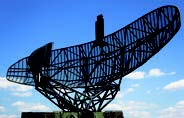
\includegraphics{4-25.pdf}
    \caption{火车车轮有凸出的轮缘}\label{fig:4-25}
  \end{minipage}
  \begin{minipage}[b]{0.48\linewidth}
    \centering
    \includegraphics{4-26.pdf}
    \caption{外轨作用在轮缘上的力指向圆心}\label{fig:4-26}
  \end{minipage}
\end{figure}

大家注意过吗?火车的车轮上有凸出的轮缘(\cref{fig:4-25})。
当火车在平直轨道上匀速行驶的时候,轮缘并不与铁轨相互作用。
在火车转弯处,如果内外轨一样高,外侧车轮的轮缘就挤压外轨,轮缘和铁轨都发生弹性形变,而产生相互作用的弹力。
外轨作用在轮缘上的弹力 $F'$,就是指向圆心使火车产生向心加速度的向心力(\cref{fig:4-26})。
如果火车转弯时的速率是 $v$,转弯处弧形轨道的半径是 $r$,火车的质量是 $m$,那么
\[F'=m\frac{v^2}{r}.\]
火车的质量和速率都相当大,$F'$ 也相当大,根据牛顿第三定律,外侧车轮的轮缘向外挤压外轨的力跟 $F'$ 大小相等、方向相反,外轨在这个力的挤压下很容易损坏。
怎样才能减小轮缘跟铁轨相互挤压的力而又能产生使火车转弯所需的向心力呢?
\begin{figure}
  \includegraphics{4-27.pdf}
  \caption{外轨高于内轨时,重力与支持力的合力指向圆心}\label{fig:4-27}
\end{figure}

我们可以使路面向圆心一侧倾斜一个很小的角度,使外轨略高于内轨(\cref{fig:4-27}),这时支持力 $N$ 不再与重力 $G$ 平衡,它们的合力 $F$ 指向圆心。
这个合力 $F$ 和外轨对轮缘的弹力 $F'$ 的共同作用,使火车产生向心加速度 $v^2/r$。
可见外轨略高于内轨时能减小外轨与轮缘间的作用力。

如果外轨超出内轨的高度适当,可以使重力 $G$ 与支持力 $N$ 的合力 $F$ 刚好等于火车转弯所需要的向心力 $mv^2/r$。这时 $F'=0$,即外轨与轮缘不相互挤压。
在修筑铁路的时候,正是根据转弯处轨道的半径 $r$ 和规定的行驶速率 $v$,选择适当的路面倾斜角度 $\alpha$,或者说选择适当的内外轨高度差 $h$,来使 $F'=0$。
对于已经修筑好的铁路,转弯处的 $r$ 和 $h$ 已经定了,如果火车速率超过规定的速率,$F$ 将小于需要的向心力,所差的仍需由外轨对轮缘的弹力来弥补。
如果火车的速率小于规定的速率,$F$ 将大于需要的向心力,超出的则由内轨对内侧车轮轮缘的弹力来平衡。

\begin{Practice}
\begin{question}
	\item 在\cref{fig:4-24} 的圆锥摆中,如果线和垂直方向成 \ang{30} 角,小球在水平面内做每分钟 60 转的匀速圆周运动,线的长度是 \qty{0.28}{m},计算重力加速度的值。
\item 有人说:“\cref{fig:4-24} 中的圆锥摆少画了一个作用在小球上的力,这个力与$F$ 大小相等、方向相反,是 $F$ 的平衡力,必须有这个力,小球才能处于平衡状态而不落向圆心。”这种说法错在哪里?
\item 铁路转弯处圆弧的半径是 \qty{300}{m},轨距是 \qty{1435}{mm},规定火车通过这里的速度是 \qty{72}{km/h},计算内、外铁轨的高度差。
\item 一架滑翔机用 \qty{180}{km/h} 的速率,沿着半径为 \qty{1200}{m} 的水平圆弧飞行,计算机翼和水平线的夹角(参阅\cref{fig:4-22})。
\end{question}
\end{Practice}

\section{离心现象}
\subsection{离心运动} 
要使质量是 $m$ 的物体以角速度 $\omega$ 沿半径是 $r$ 的圆周运动,就要使物体受到大小等于 $m\omega^2r$ 的向心力。
当角速度 $\omega$ 增大时,要保持物体到圆心的距离 $r$ 不变,所需的向心力必须增大,这就要相应地增大作用在物体上的合外力。
但是合外力不是可以无限增大的。
例如\cref{fig:4-21} 所示的物体做匀速圆周运动需要的向心力,是由绳的弹力提供的,弹力是由绳的形变产生的。
物体绕圆心旋转的角速度增大时,绳的拉伸形变必须随着增大,这样才能提供足够大的向心力使物体做圆周运动。
但绳的拉伸是有限度的。
当角速度增大到一定程度时,绳会被拉断,弹力 $F$ 就突然消失,这时物体将因惯性沿圆周的切线飞出(\cref{fig:4-28}),离圆心越来越远。
同样,如果作用在物体上的合外力 $F$ 小于它做匀速圆周运动所需的向心力即 $F<m\omega^2 r$,物体也不能继续沿原来的圆周轨道运动,而要沿着一条曲线运动,离圆心越来越远(\cref{fig:4-28})。
\begin{figure}
  \includegraphics{4-28.pdf}
  \caption{向心力突然消失或向心力不足时物体的离心运动}\label{fig:4-28}
\end{figure}

\emph{做匀速圆周运动的物体,在合外力突然消失或者合外力不足以提供所需的向心力时将做逐渐远离圆心的运动,这种运动叫做}\Concept{离心运动}。

\subsection{离心机械}

利用离心运动的机械叫做离心机械。
离心机械的种类很多,应用很广,下面介绍离心脱水器和离心转速计。

离心脱水器是用来甩掉湿物体上的水的装置。
洗衣机里的脱水筒,纺织厂里使湿的棉纱、毛线或纺织品脱水的器械,就是这种装置。

离心脱水器的主要部分是一个可以转动的筒,篱壁上有许多小孔(\cref{fig:4-29}),湿物体就放在这个筒里。
当筒转动得相当快的时候,水滴跟物体间的附着力小于水滴做圆周运动需要的向心力,于是水滴离开物体,逐步远离圆心,到达筒边,穿过小孔,因惯性面沿切线飞出,这样就把湿物体上的水甩掉了。

\begin{figure}
	\begin{minipage}[b]{0.48\linewidth}
		\centering
    \includegraphics{4-29.pdf}
    \caption{离心脱水器}\label{fig:4-29}
	\end{minipage}
	\begin{minipage}[b]{0.48\linewidth}\centering
    \includegraphics{4-30.pdf}
    \caption{离心转速计}\label{fig:4-30}
	\end{minipage}
\end{figure}

离心转速计是用来测量机器转速的一种仪器,它的构造如\cref{fig:4-30} 所示。
在转速计的转轴 $OO'$ 上的 $E$ 处安装着一根轻的金属棒,棒的两端有两个重球 $m_1$ 和 $m_2$,金属棒可以绕 $E$ 点转动,弹簧 $L_1$ 和 $L_2$ 用来把金属棒拉向转轴。
滑套 $K$ 可以沿转轴上下移动。
把转速计的转轴 $OO'$ 跟机器的转轴连接在一起,当机器的轴转动时,$OO'$ 随着转动,重球 $m_1$ 和 $m_2$ 跟着做圆周运动,所受的向心力是由弹簧的拉力提供的。
轴转动得越快,重球做圆周运动的半径就越大。滑套 $K$ 在轴上就上升得越高,同时带动指针向左偏转,从刻度盘上就可以读出机器的转速。

\subsection{一些有害的离心运动} 

离心运动有时会造成危害,需要设法防止。
高速转动的砂轮、飞轮,都不得超过允许的最大转速,如果转速过高,砂轮、飞轮内部的相互作用力小于需要的向心力,砂轮、飞轮某些组成部分的离心运动会使它们破裂,高速甩出后可能酿成事故。
飞机由俯冲拉起时或者飞机翻斤斗时,飞行员的血液由于离心运动向下肢流去,造成飞行员大脑贫血,四肢沉重,这种现象叫做过荷。
过荷太大时,飞行员就会暂时失明,甚至晕厥。
在飞行训练和空战时过荷现象是难免的,飞行员可以依靠加强训练、增强体质来提高自己的抗荷能力。
\cref{fig:4-31} 是离心试验器的原理图,它用来研究过荷对人体的影响,测验人的抗荷能力。
\begin{figure}
  \includegraphics{4-31.pdf}
  \caption{离心试验器}\label{fig:4-31}
\end{figure}

\begin{Review}
\begin{question}
	\item 物体做曲线运动的条件是什么?做曲线运动的物体在任一时刻的即时速度方向是什么?为什么说曲线运动总是变速运动?
  \item 什么叫运动的合成,什么叫运动的分解?怎样进行运动的合成和分解?
  \item 平抛运动可以看做是哪两个运动合成的?它的运动轨迹是什么曲线?怎样确定平抛物体在任一时刻的位置?
  \item 斜抛运动是由哪两个分运动合成的?它的运动轨迹是什么曲线?斜抛运动跟竖直上抛运动和平抛运动之间有什么关系?怎样确定斜抛物体在任一时刻的位置?怎祥确定斜抛物体的射高和射程?在什么情况下斜抛物体的射程最大?
  \item 什么是匀速圆周运动?描述匀速圆周运动的快慢有哪几个物理量,它们之间的关系是怎样的?
  \item 为什么做匀速圆周运动的物体需要有一个向心力?在分析做圆周运动物体的受力情况时,有的同学往往错误地认为,这个物体除了受到另外物体对它的作用力,还受到一个向心力。这样来分析,为什么是错误的?复习课文中讲过的和你自己做过的分析向心力的实例,并加以总结。
  \item 怎样计算向心加速度和向心力的大小?物体的向心加速度和所受的向心力跟哪些因素有关系?写出向心加速度和向心力的不同形式的公式,并说明它们之间的关系和各自的物理意义。
  \item 什么叫离心运动?试举一两个例子说明它的应用。
\end{question}
\end{Review}


\begin{Exercise}*
\begin{question}
	\item 汽艇在静水中的速度是 \qty{10}{km/h},渡河时向着垂直于河岸的方向匀速行驶。现在河水的流速是 \qty{3}{km/h},河宽 \qty{500}{m},汽艇驶到对岸需要多长时间?汽艇在河水中实际行驶的距离是多大?
  \item 在 \qty{490}{m} 的高空,以 \qty{240}{m/s} 的速度水平飞行的轰炸机,追击一鱼雷艇,该艇正以 \qty{25}{m/s} 的速度与飞机同方向行驶。试问,飞机应在鱼雷艇后面多远处投下炸弹,才能击中该艇?
  \item 两人传球,如果球从一个人手里到另一个人手里经过的时间是 \qty{2}{s},球到达的最高点离手有多高?(设两人的手等高)
  \item 从仰角是 \ang{30} 的枪筒中射出的子弹,初速度是 \qty{600}{m/s} 。求子弹在轨迹最高点和落地点的速度各是多大。
  \item 伽利略曾说过:“仰角(即抛射角)比\ang{45} 增大或减小一个相等角度的抛体,其射程是相等的。”你能证明这个说法的正确性吗?
\item 一个人站在地面上用枪瞄准树上的猴子(\cref{fig:4-32}),当子弹从枪口射出时,猴子闻声立即从树上竖直下落(初速度为零)。讨论一下,猴子能否避开子弹的射击。

提示:斜抛运动可以看作是物体沿初速度方向所做的匀速直线运动和在重力作用下的自由落体运动的合运动。

\begin{figurehere}
  \includegraphics{4-32.pdf}
  \captionof{figure}{}\label{fig:4-32}
\end{figurehere}

\item  飞机从俯冲到拉起的一段轨迹是一段圆弧(参看\cref{fig:4-19}),如果飞机在这段弧上的速率是 \qty{540}{km/h},要使它在最低点时的向心加速度不超过 $5g$,圆弧的半径至少是多少米?($g$ 取 \qty{10}{m/s^2})。
\item  一个 \qty{35}{kg} 的重物,系在 \qty{2.0}{m} 长的悬绳下端,不断摆动。重物通过最低点时的速率是 \qty{3.0}{m/s},求这时绳对物体的拉力。
\item  要使小球滑到圆形轨道顶端时不掉下来(\cref{fig:4-33}),小球在轨道顶端的最小速率应是多大?已知圆形轨道的半径为 $R$。
\begin{figurehere}
  \begin{minipage}{\linewidth}\centering
    \includegraphics{4-33.pdf}
    \captionof{figure}{}\label{fig:4-33}
  \end{minipage}
\end{figurehere}

% \begin{solution}
% 小球在圆形轨道顶端时受到的力有两个:重力和轨道对小球的压力,它们的方向都是竖直向下的。这两个力的合力就是小球做圆周运动通过轨道顶端时所受的向心力。小球受到的重力是固定不变的,轨道对小球的压力跟小球通过轨道顶端时的速率有关系,速率越小,小球所需的向心力越小,轨道对小球的压力就越小。当速率小到某一数值时,轨道的压力减为零,小球所需的向心力仅由重力提供,这个速率就是
% 小球滑到轨道顶端时不掉下来的最小速率。如果速率再小,
% 小球所需的向心力小于它受到的重力,小球将脱离圆形轨道而掉下来。

% 设小球通过轨道顶端时的最小速率为$v$,这时小球所需
% 的向心力等于$mv^2/R$。
% 由以上的分析可知,要使小球不掉下来,
% 向心力必须满足下式:\[m\frac{v^2}{R}=mg \]
% 所以\[v=\sqrt{Rg} \]
% \end{solution}

\item  一个滑雪者连同他的滑雪板质量共 \qty{70}{kg},他滑到凹形的坡底时的速度是 \qty{20}{m/s},坡底的圆弧半径是 \qty{50}{m},计算在坡底时雪地对滑雪板的支持力。
\item  一辆 \qty{600}{kg} 的汽车以 \qty{10}{m/s} 的速度通过圆弧半径是 \qty{30}{m} 的山坡顶点时,汽车受到哪几个力的作用?汽车对路面的压力是多大?
\end{question}
\end{Exercise}